\section{Experiments} \label{sec:experiments}
       
\subsection{Datasets} \label{sec:dataset}

\paragraph{DeepFashion2}

\begin{figure} [H]
    \centering
    \captionsetup{justification=centering}
    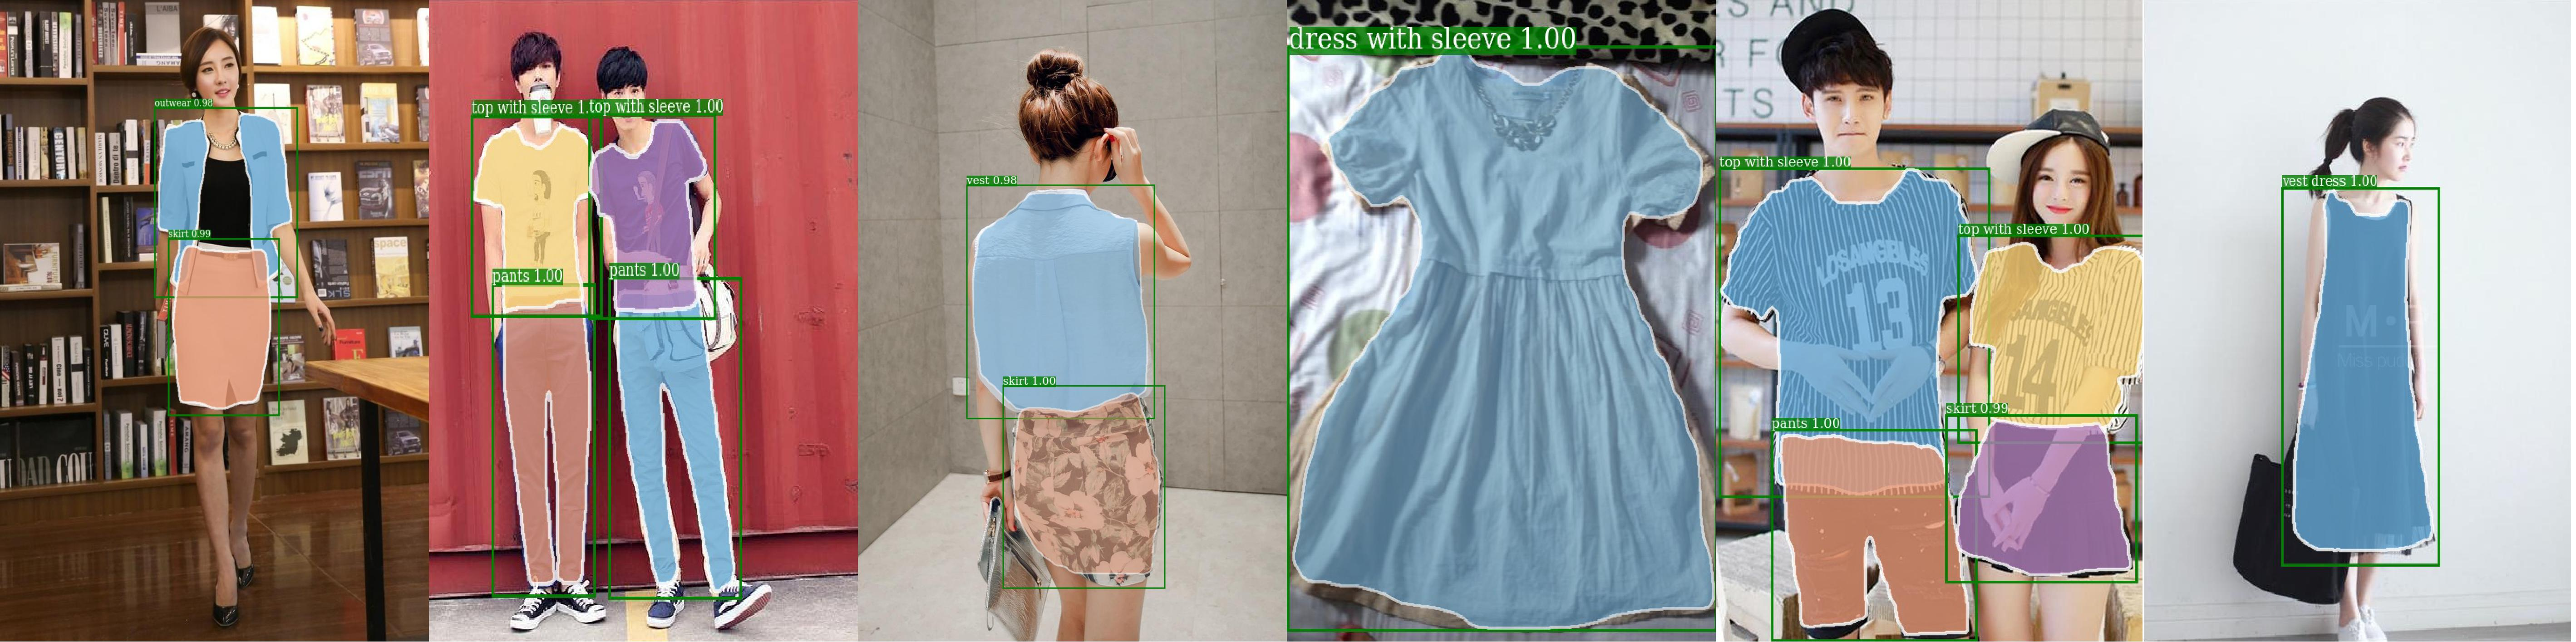
\includegraphics[width=0.9\textwidth]{chapter4/image/deepfashion20.jpg}
    \caption{Polygon annotation examples in DeepFashion2 dataset}
    \label{fig:df}
\end{figure}

DeepFashion is a large-scale clothes dataset with over 800.000 images of 46 clothing categories under different scenarios, namely street snapshot, store. DeepFashion2 is an extension of DeepFashion, proposed to study a broad spectrum of computer vision applications for fashion, including clothes retrieval, clothes recommendation, and virtual try-on. Applied for comprehensive tasks, DeepFashion2 has richer annotations such as style, bounding box, viewpoint, scale, etc. It contains 491.000 images of 13 clothing categories. Here is the identity number and name of the whole thirteen categories: 1 represents short sleeve top, 2 represents long sleeve top, 3 represents short sleeve outwear, 4 represents long sleeve outwear, 5 represents vest, 6 represents sling, 7 represents shorts, 8 represents trousers, 9 represents skirt, 10 represents short sleeve dress, 11 represents long sleeve dress, 12 represents vest dress and 13 represents sling dress. \par 

\begin{figure} [H]
    \centering
    \captionsetup{justification=centering}
    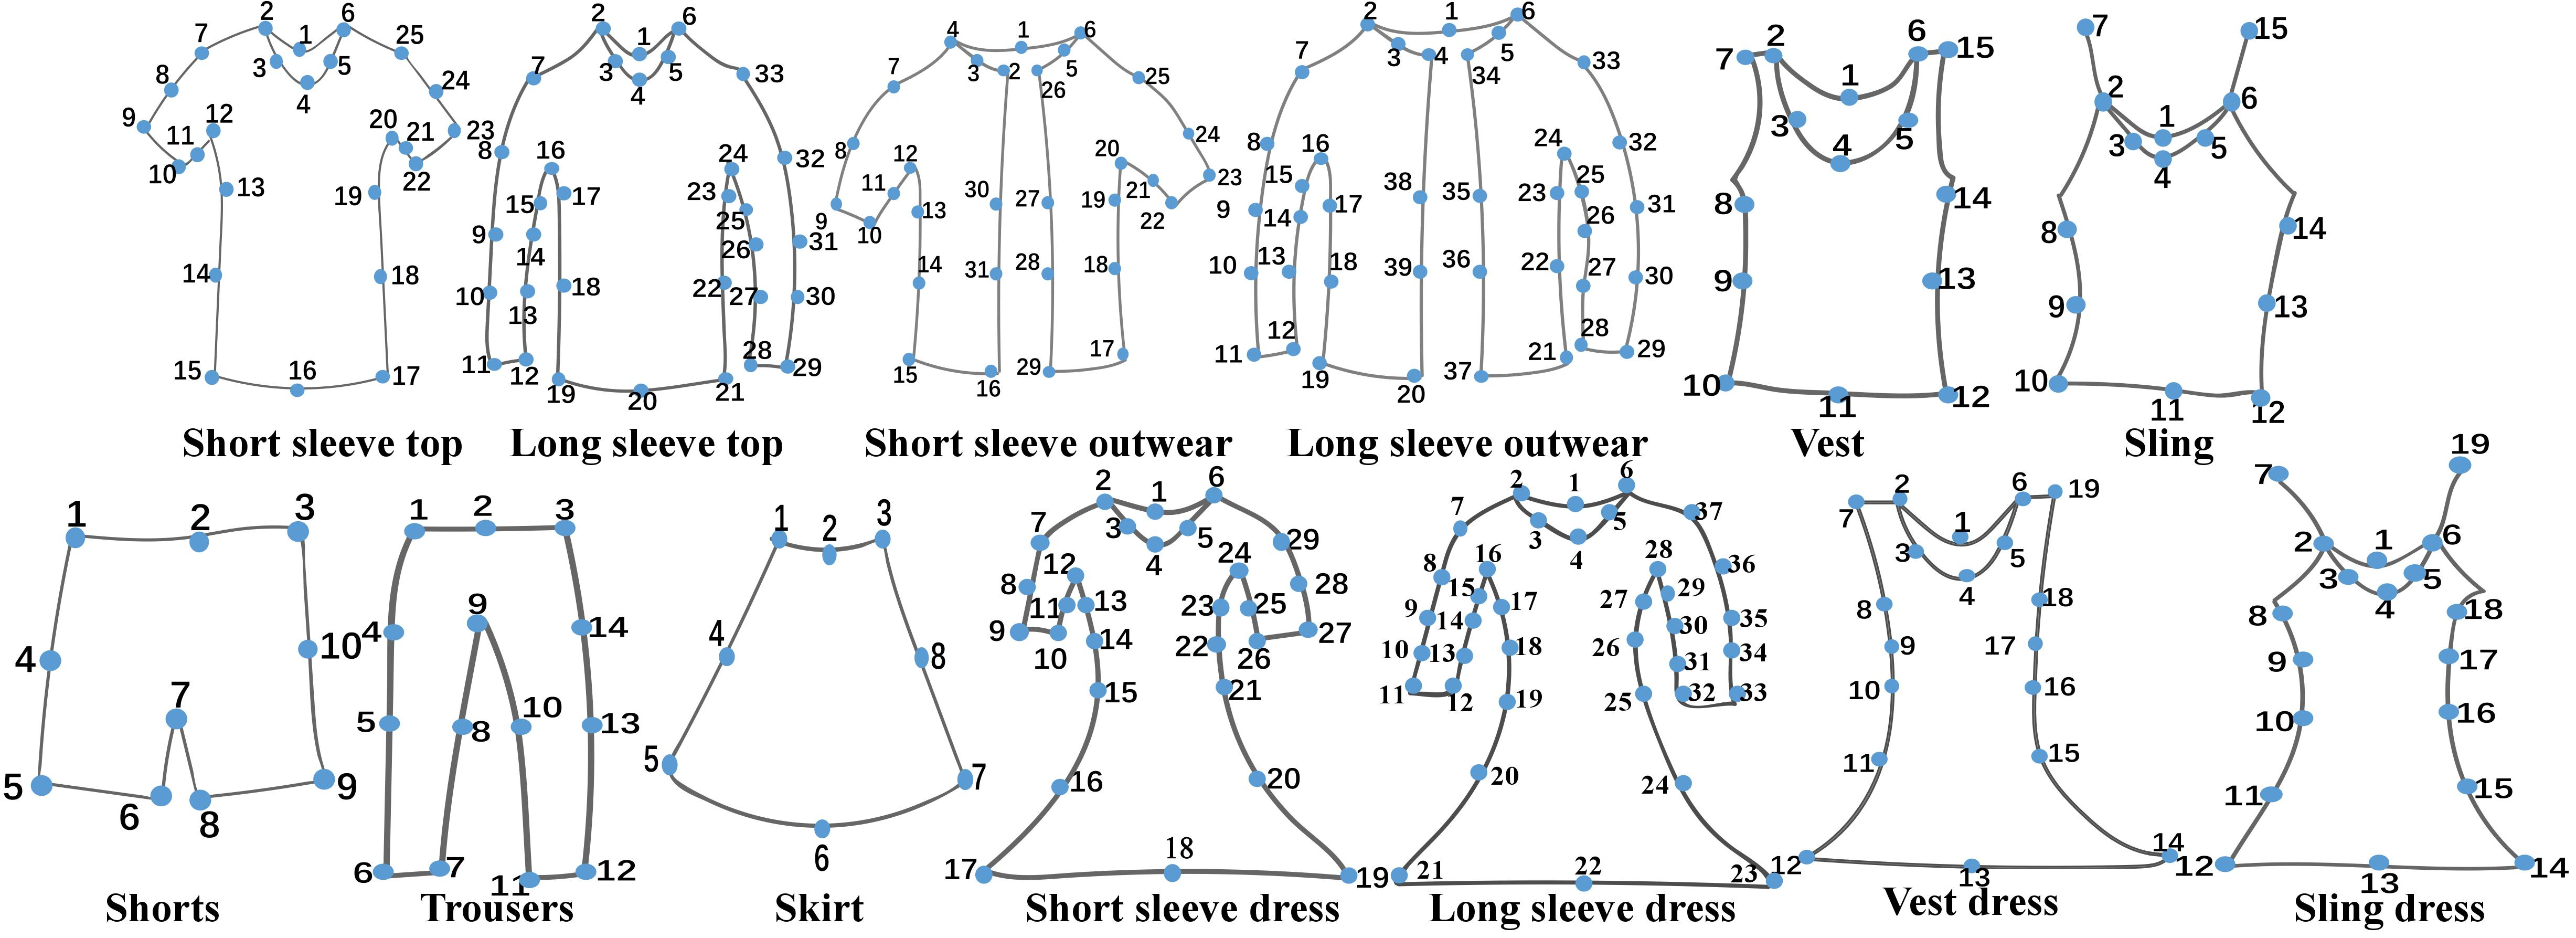
\includegraphics[width=0.9\textwidth]{chapter4/image/deepfahsion2_class.jpg}
    \caption{Thirteen categories of DeepFashion2 dataset}
    \label{fig:dfcate}
\end{figure}

However, I only use the dataset for upper-body clothes (includes the first six categories) recognition. Thus images with categories from 6 to 13 are excluded. After removing lower-body clothes, the dataset remains 137,850 images in the training set. \par


\noindent Differences when compare DeepFashion2 with DeepFashion:
\begin{itemize}
\item DeepFashion2 includes multiple items (pieces of clothing) in an image, while DeepFashion only has a single item per image.
\item DeepFashion is annotated with sparse landmarks per, each piece of cloth only has from 4 to 8 landmarks. In DeepFashion2, each item is manually labeled. With bounding box, mask, dense landmark (20 per item on average)
\item DeepFashion annotations are stored in text files, while DeepFashion2 annotations are stored in JSON format files.
\end{itemize}


\paragraph{Figaro1k}

Figaro1k is the first multi-class hair database where images are organized in the following classes: straight, wavy, curly, kinky, braids, dreadlocks, and short-men, each containing 120 images. \par

\begin{figure} [H]
    \centering
    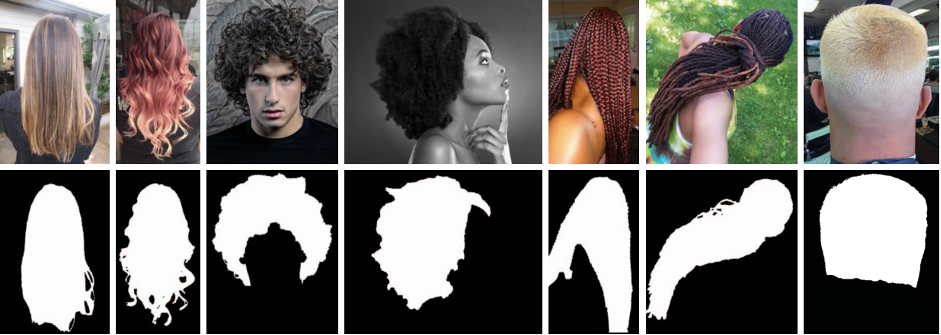
\includegraphics[width=0.9\textwidth]{chapter4/image/figaro.png}
    \caption{Examples of image and mask in Figaro1k dataset}
    \label{fig:figaro}
\end{figure}

Figaro1k consists of 1050 images, equally distributed in seven hairstyle classes. It is regarded as an annotated novel multi-class image database for hair analysis in the wild.

\paragraph{LFW}
LFW,  stands for "Labeled Faces in the Wild", is also an annotated face dataset in the wild dataset. It contains more than 2,000 images of faces collected from the web. Each face has been labeled with the name of the person pictured so that the dataset is also used as the benchmark for the face recognition problem.

\begin{figure} [H]
    \centering
    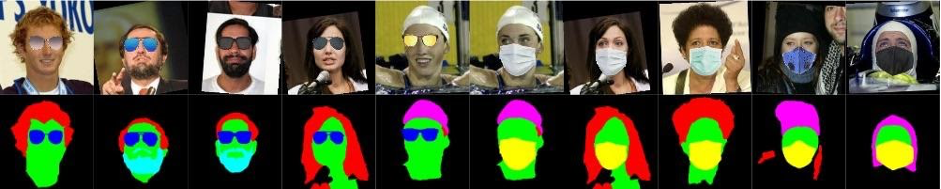
\includegraphics{chapter4/image/lfw.png}
    \caption{Examples of image and mask in LFW dataset}
    \label{fig:lfw}
\end{figure}

Each image is a JPG image with the size of 250x250. The dataset is already split into train, validation, and test set. They have respectively 1500 images, 500 images, and 900 images.
       
\subsection{Data preparation}

In a segmentation task, it is typically challenging to obtain an adequate training set of annotated data. The process of annotation is time-consuming, even when support tools are supplied. However, I used three publicly available datasets: DeepFashion2 for the clothes segmentation task, Figaro1k and LFW for the hair segmentation task. All of them are provided publicly; they have already been attached to annotations. However, they are organized differently. \par

\paragraph{DeepFashion2}
DeepFashion2 is a massive dataset; it has already been divided into the training set, validation set, and test set. The training set has 137.000 images stored in \emph{/image} folder and corresponding annotations located in \emph{/annos} folder, which is adequate for training a deep learning model. However, as the dataset's size is quite big, I read all annotation information and represent them on a Pandas DataFrame. Therefore, the dataset is highly manipulated, and I can easily filter out all data with category\_id bigger than six (because the model only aimed at upper-body clothes recognization). \par

\begin{figure} [H]
    \centering
    \captionsetup{justification=centering}
    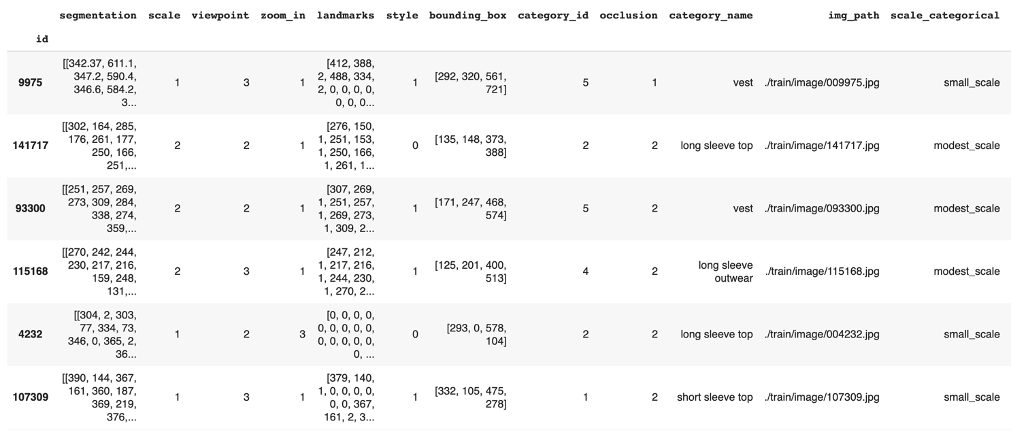
\includegraphics[width=0.9\textwidth]{chapter4/image/dataframe.png}
    \caption{Head of DataFrame of DeepFashion2’s trainning set}
    \label{fig:df}
\end{figure}

The above figure depicts the format of a DataFrame after synthesized from many JSON annotation files. Each row corresponding to an image has information like image path, category, polygons segmentation… \par

\paragraph{Figaro1k and LFW}
Figaro1k and LFW are organized into an image folder and an annotation folder. The image folder consists of images under \emph{jpg} extension, while the annotation folder consists of annotations under the bpm extension. Thus, it is more straightforward to read these two datasets when compared to DeepFashion2. Plus, these two datasets are much more lightweight than DeepFashion2. I use OpenCV2 to encode all images and their corresponding annotations; it outputs a Numpy array, which can forward instantly through the neural network. \par

\subsection{Data augmentation}
Data augmentation is the process of enriching the dataset by applying some transformations to the initial image to generate augmented images. It acts as a regularizer or to speed up convergence, thereby avoid overfitting and improve generalization capabilities. Some image transform operations used in the work are collectively horizontal and vertical flipping, 90-degree rotation, CLAHE, RandomContrast, and RandomGamma. \par

\begin{figure}[H]
    \centering
    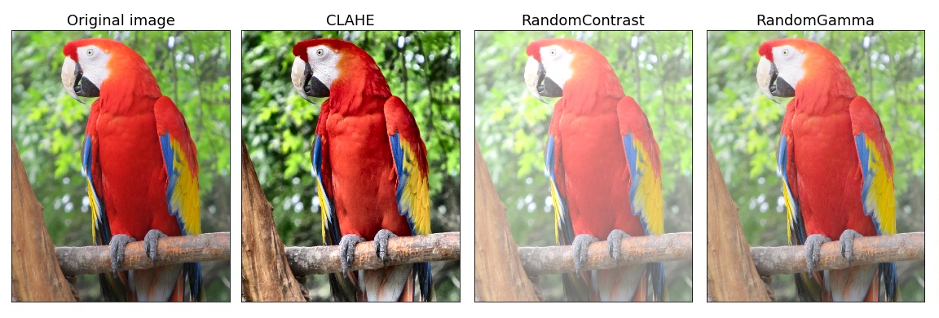
\includegraphics{chapter4/image/augmentation.png}
    \caption{Illustration for transform operations}
    \label{fig:augmentation}
\end{figure}

All of the transformations are composed and applied separately to each image in the dataset with specific probabilities; hence the transformations are guaranteed to apply randomly. As a result, the network sees different data each epoch, and this would generalize the model. \par
I use the Albumentations library \cite{albumentations}, a Python library, to handle the entire augmentation process.


\subsection{Trainning}

The proposed CNN, introduced in \textbf{section \ref{sec:model}}, is implemented by using the Tensorflow framework. The environment used for training is CoLab Pro with 25 GBs of memory, 16 GBs of GPU, and 147 GBs of disk. While the base network load weights pre-trained in the ImageNet dataset, the weights of the rest of the model are initialized randomly.
\par 
The model for hair segmentation is trained in the LFW and Figaro1k dataset with Adam optimization with $\beta_{1} = 0.9$ and $\beta_{2} = 0.999$. The learning rate is set to 1e-3, the batch size is 16. The model is trained for 46 epochs with all parameters trainable.
\par
Meanwhile, the model for clothes segmentation is trained in the DeepFashion2 dataset with Adam optimization with $\beta_{1} = 0.9$ and $\beta_{2} = 0.999$. The learning rate is set to 1e-3, the batch size is 64. The network is trained for 15 epochs. For the first 10 epochs, the base network is frozen. Later, it is unfreezing in the latter 5 epochs.
\par
